%%%%%%%%%%%%%%%%%%%% author.tex %%%%%%%%%%%%%%%%%%%%%%%%%%%%%%%%%%%
%
% sample root file for your "contribution" to a proceedings volume
%
% Use this file as a template for your own input.
%
%%%%%%%%%%%%%%%% Springer %%%%%%%%%%%%%%%%%%%%%%%%%%%%%%%%%%

%%%%%%%%%%%%%%%%%%%%%%%%%%%%%%%%%%%%%%%%%%%%%%%%%%%%%%%%%%%%%%%5
%% 

%   http://2023.cisisconference.eu/important-dates/

%%  Tope 10 paginas
%%  http://2023.sococonference.eu/paper-submission-publication/

%%%%%%%%%%%%%%%%%%%%%%%%%%%%%%%%%%%%%%%%%%%%%%%%%%%%%%%%%%%%%%%%

\documentclass{svproc}


%%% PAQUETES  %%%
%%% PAQUETES  %%%

%%% Soporte extendido de colores
\usepackage{xcolor}
    % Definiciones colores extra
    %% Ref: http://latexcolor.com/
    \definecolor{coolblack}{rgb}{0.0, 0.18, 0.39}
    \definecolor{dimgray}{rgb}{0.41, 0.41, 0.41}

%%% Paquete para poner hipervinculos más finos \href
\PassOptionsToPackage{hyphens}{url}
\usepackage{hyperref}

   %Colores personalizados
    \hypersetup{
        colorlinks=true,
        linkcolor=black,
        filecolor=black,
        %%% Necesita su propia definicion de color
        citecolor=dimgray,
        urlcolor=coolblack,
    }

%%% Formato y tipografía de URL, direcciones de correo...
\usepackage{url}
    \def\UrlFont{\rmfamily}

%%% Usados por graficas de barras
\usepackage{textcomp}
\usepackage{tikz}
\usepackage{pgfplots}
\usepackage{pgfplotstable} 
\usepackage{csvsimple}% Generates table from .csv
\pgfplotsset{compat=1.7}
\usepackage{subcaption}
\usepgfplotslibrary{groupplots}

% PGFPlots Settings
\pgfplotsset{
SmallBarPlot/.style={
    font=\footnotesize,
    ybar,
    width=\linewidth,
    ymin=0,
    xtick=data,
    xticklabel style={text width=1.5cm, rotate=90, align=center}
},
BlueBars/.style={fill=blue!20, bar width=0.25},
RedBars/.style={fill=red!20, bar width=0.25},
GreenBars/.style={fill=green!20, bar width=0.25}
}

%% Para incluir en el texto o en el pie de la figura la leyenda con colores.
\DeclareRobustCommand\legendbox[1]{(\textcolor{#1}{#1 bars}~\begin{tikzpicture}[x=0.2cm, y=0.2cm] \draw [color=black, fill=#1!20] (0,0) -- (0,1) -- (0.6,1) -- (0.6,0) -- (0, 0); \end{tikzpicture})}

\usepackage{booktabs} % usado en tablas generadas con JASP


%%%%%%%%%%%%%%%%%%%%%%%%%%%%%%% HEREDADOS JNIC %%%%%%%%%%%%%%%%%%%%%%%%%%%%%%%

%%% TODO NOTES y definición 2cm de margen para que no se solapen añadido colores comentarios
 \setlength {\marginparwidth }{2cm} 
 \usepackage{todonotes}
 \usepackage[normalem]{ulem}

%%% Paquete para comentarios
\usepackage{verbatim}

%%% Tildes y demás caracteres en castellano...
%\usepackage[latin1]{inputenc}
% o bien
\usepackage[utf8]{inputenc}

%%% Fuente Times...
\usepackage{times}

%%% Figuras en formato .png, .ps, pdf o eps
\usepackage{graphicx}
%%\usepackage{subfigure}
\DeclareGraphicsExtensions{.png,.eps,.ps,.pdf}

%%% Soporte graficos svg
\usepackage{svg}

%%% Sección para definir explícitamente la separación de sílabas al final de una línea:
\hyphenation{si-guien-do}

%%% Secciones etc. en castellano
%\usepackage[spanish,es-tabla]{babel}

%%% Secciones etc. en Ingles
\usepackage[english]{babel}


%%% Paquete para usar simbolos y scripts de dibujado
\usepackage{tikz}
\def\checkmark{\tikz\fill[scale=0.4](0,.35) -- (.25,0) -- (1,.7) -- (.25,.15) -- cycle;} 
\usetikzlibrary{shapes,arrows}

% Define Block styles
\tikzstyle{decisionBL} = [diamond, draw, fill=blue!20,text width=10em, text badly centered, node distance=3cm, inner sep=0pt]
\tikzstyle{blockBL} = [rectangle, draw, fill=blue!20,text width=9em, text centered, rounded corners, minimum height=4em]
\tikzstyle{blockYL} = [rectangle, draw, fill=yellow!20, text width=9em, text centered, rounded corners, minimum height=4em]
\tikzstyle{blockGR} = [rectangle, draw, fill=green!20, text width=9em, text centered, rounded corners, minimum height=4em]
\tikzstyle{blockRD} = [rectangle, draw, fill=red!20, text width=9em, text centered, rounded corners, minimum height=4em]
\tikzstyle{blockWH} = [rectangle, draw, fill=white!20, text width=9em, text centered, rounded corners, minimum height=4em]
\tikzstyle{line} = [draw, -latex']
\tikzstyle{cloud} = [draw, ellipse,fill=red!20, node distance=4.5cm,minimum height=4em]

%%% Para usar ficheros tex de infografias Inkscape
\usepackage{pstricks}
\usepackage{comment}    
%%% COMANDOS  %%%
%%% COMANDOS  %%%

%%% A cursiva  %%%
\newcommand{\cursiva}[1]{\em{#1}}


%%% Fuzzing en bonito  %%%
\newcommand{\fz}{\em fuzzing}

%%% Atajos estilo  %%%

\newcommand{\CLASSINPUTinnersidemargin}{18mm}
\newcommand{\CLASSINPUToutersidemargin}{12mm}
\newcommand{\CLASSINPUTtoptextmargin}{20mm}
\newcommand{\CLASSINPUTbottomtextmargin}{25mm}

\newcommand{\new}[1]{\textcolor{olive}{{#1}}}
%\newcommand{\old}[1]{\textcolor{purple}{{\sout{#1}}}}
\newcommand{\wip}[1]{\textcolor{blue}{{#1}}}
%\newcommand{\checkthis}[1]{\textcolor{orange}{{#1}}}
\newcommand{\diego}[1]{\textcolor{magenta}{{#1}}}
\newcommand{\vmodixit}[1]{\textcolor{teal}{{#1}}}

\newcommand{\old}[1]{\textcolor{purple}{{\sout{#1}}}}
\newcommand{\camino}[1]{\textcolor{olive}{{#1}}}
\newcommand{\fjrodl}[1]{\textcolor{blue}{{#1}}}
\newcommand{\checkthis}[1]{\textcolor{orange}{{#1}}}

%%% Entornos  %%%
\newcounter{definicion}
\newenvironment{definicion}[1]{%
    \refstepcounter{definicion}\par\medskip%
    \noindent \textbf{Definición~\thedefinicion. #1}.\ %
}{\medskip}

%%%% Soporte para el logo de ORCID
%\newcommand{\orcid}[1]{\href{https://orcid.org/#1}{\textcolor[HTML]{A6CE39}{\aiOrcid}}}



\begin{document}
\mainmatter              % start of a contribution
%
%Impacto de Aproximaciones Distribuidas en HPC al {\fz} de ROS 2
\title{Fuzzing Robotic Software using HPC}
%
\titlerunning{{\fz} in ROS 2}  % abbreviated title (for running head)
%                                     also used for the TOC unless
%                                     \toctitle is used


% Soporte logo orcid
% Depepende de \usepackage{svg}
\newcommand{\orcid}[1]{\href{https://orcid.org/#1}{
\includegraphics[width=8pt]{figures/data/orcid_logo.png}}}




\author{
  Francisco Borja Garnelo Del Río \orcid{0000-0002-8935-0669} \and
  Francisco J. Rodríguez Lera \orcid{0000-0002-8400-7079} \and  
  Camino Fernández Llamas \orcid{0000-0002-8705-4786} \and
  Vicente Matellán Olivera \orcid{0000-0001-7844-9658}
  }



\authorrunning{Francisco Borja Garnelo et al.} % abbreviated author list (for running head)
%
%%%% list of authors for the TOC (use if author list has to be modified)
\tocauthor{Francisco Borja Garnelo Del Río, Francisco J. Rodríguez Lera, Camino Fernández Llamas, Vicente Matellán Olivera}
%


\institute{Universidad de León, Campus de Vegazana s/n, 24071 León , Spain,\\
\email{\href{mailto:infbgd01@estudiantes.unileon.es}{infbgd01@estudiantes.unileon.es}, \\ \href{mailto:fjrodl@unileon.es;cferll@unileon.es;vmato@unileon.es}{\{fjrodl, cferll, vmato\}@unileon.es}}
,\\ WWW : \texttt{\url{https://robotica.unileon.es/}}}



\maketitle              % typeset the title of the contribution

%%% RESUMEN  %%%%
% Entre 70 y 150 palabras
\begin{abstract} 
Developing secure systems is particularly important in autonomous systems, where testing and debugging robotic platforms are very complex. This paper presents a novel HPC pipeline for fuzzing robotic software systems that control robots. 
Speeding up the fuzz process allows more testing to be performed in less time. By using parallel processing, HPC systems can perform computations much faster and more efficiently than traditional personal computers, in this way, the paper presents an updated version of the fuzzing pipeline for HPC environments. 
To validate the pipeline, a containerized version of the sota fuzzer RoboFuzz has been implemented for running in HPC, and to empirically evaluate its performance against a personal computer and the original approach. The full empirical approach is available to other researchers on GitHub.

\keywords{Robotics,{\fz},HPC, RoboFuzz, Software security, Singularity, ROS 2, Simulation}

\end{abstract}
%

\section{Introduction}


Fuzz testing, also known as fuzzing, was first used in a study of UNIX security in the 1990s~\cite{inicio_fuzzing,continuacion_fuzzing}. It is a highly effective software testing technique employed to discover security vulnerabilities, programming errors, and other potential issues in software systems. By subjecting the target system to a multitude of random, malformed, or unexpected input data, fuzzing aims to provoke unanticipated responses, crashes, or unexpected behaviors, thus revealing weaknesses that can be exploited or lead to system instability. 

Fuzz testing techniques can be applied to evaluate the robustness and security of the software components governing the robot's operation\cite{rvfuzzer}. Robotic systems typically consist of numerous interconnected modules such as control algorithms, sensor data processing, communication protocols, and user interfaces. The complexity of these systems makes them highly susceptible to software bugs and vulnerabilities, which can lead to malfunctions or even catastrophic failures, thus having a high impact these days on robots, for instance, in collaborative environments.

Fuzz testing in robotics can be applied at various levels of granularity, from individual components or modules to the entire system. For instance, fuzzing can be used to test the robustness of specific algorithms, such as localization or path planning, by providing them with unexpected or corrupt sensor data. At a higher level, fuzz testing can be applied to the communication protocols and data exchange between different modules within a robotic system, simulating failures or attacks on the communication channels.
Thus, it is necessary to speed up the process of evaluating any piece of source code that can be deployed in the robot.
Complex tasks or algorithms with large datasets should be tested in reasonable windows of time, which leads to the use of High-Performance Computing (HPC) systems.


HPC can significantly enhance the fuzzing testing process by providing the computational resources and parallel processing capabilities needed to efficiently explore the vast input space of complex systems, such as those found in robotics. The use of HPC for fuzzing testing can lead to improvements in several key aspects of the fuzzing process:

\begin{itemize}
    \item  Scalability: Fuzz testing can generate a large number of test inputs, and processing these inputs can be computationally expensive, especially for complex systems. HPC  provides the necessary computing power to enable parallel execution of test cases, which dramatically increases the scalability of the fuzzing process.
    \item   Speed: By leveraging the parallel processing capabilities of HPC systems, fuzz testing can be performed much faster than in traditional single-node systems. 
    \item  Real-time monitoring and analysis: The use of containers on HPC enables real-time monitoring and analysis of the fuzz testing process, providing researchers with insights into the system's behavior and vulnerabilities as they are discovered. This can help guide the testing process, enabling more targeted and effective testing strategies.
    \item  Large-scale simulations: HPC resources can be used to run large-scale simulations of complex robotic systems, allowing for more realistic and comprehensive fuzz testing scenarios.
    \item  Enhanced collaboration: HPC resources often come with advanced collaborative tools and frameworks, enabling researchers and developers from different locations to collaborate more effectively on fuzz testing projects. This can lead to better knowledge sharing, faster identification of vulnerabilities, and more efficient development of fixes and patches.
\end{itemize}
  
Different authors have proposed the use of HPC in robotics. Camargo et al.~\cite{camargo2018towards} have proposed an HPC-ROS package for enhancing robot performance in different run-time robot processes. Arumugam et al.~\cite{arumugam2010davinci}  use HPC to parallelize the FastSLAM algorithm using a Hadoop system.  
In the same way, this work presents how state-of-the-art fuzzing tools for Robot Operating System (ROS) can be used in HPC systems. This means that fuzzing could be included as part of the test and simulation phase of a robotic DevOps flow \cite{mayoral2020devsecops}. 


\subsection{Contribution and Hypotheses}

The goal of this paper is to provide a set of empirical evidence to categorize and assess a State-Of-The-Art fuzzing tool for software developed using Robot Operating System (ROS). Thus, the research question faced in this work can be expressed as:\\


\noindent\fbox{%
    \parbox{\textwidth}{%
        What are the implications of using HPC systems when fuzzing ROS applications?
    }%
}
\newline

This question arises from the following hypothesis and questions: 

\begin{enumerate}
    \item H1: Distributing the fuzzing workload across multiple processing units can significantly increase overall fuzzer performance. 
    \item Q1: What are the key concepts associated with Fuzzing in HPC?
    \item Q2: What is the performance of the fuzzer when running in a personal computer or HPC computer?
    
\end{enumerate}

The two main contributions of this work are:
\begin{itemize}
    \item Empirical evaluations that allow us to answer the hypothesis above.
    \item A set of publicly available Singularity containers deploying a ROS 2 fuzzer. 
    \item Lessons learned of using a SOTA fuzzer in an HPC environment. 
\end{itemize}


The remainder of this paper is organized as follows. The next section presents the state of the art, focusing on the
fuzz problem. Section~\ref{sec:materials} explains the technologies explored in this research. Section
\ref{sec:results} presents the evaluation process carried out. The lessons learned in the process are summarised in Section~\ref{sec:lessons} and the paper closes with some conclusions in Section~\ref{sec:conclusions}.


\section{State of the art}

Fuzzing testing is coming along rapidly in the last two years to evaluate robotics software. Woodlief et al. \cite{woodlief2021fuzzing} present the PHYS-FUZZ tool. They aim to perform fuzzing of robotic software that integrates traditional fuzzing with the physical attributes and hazards associated with the context of mobile robots. 
Xie \cite{xie2022rozz} designed ROZZ, a multi-dimensional generation method to generate effective test cases for ROS programs. Again, they consider multiple dimensions such as configuration parameters, messages from robot sensors, or human input introduced from GUI, command lines, and ROS services. In addition, they also propose mutation strategies, which could of course be increased with machine learning approaches \cite{wang2020systematic}.  Seulbae~\cite{Seulbae:2022} illustrates the effectiveness of their tool, RoboFuzz, tested in a case study based on a robotic manipulator system and compares its performance with other state-of-the-art fuzz testing tools.

As soon as we integrated a fleet of diverse robots and have to think about robot dimensions, dynamic characteristics of the environment or estimate trajectories and control decisions, as well as introduce machine learning approaches, it would be necessary to optimize this process using HPC computing. In this sense, several researchers have been studying how to introduce HPC in the field of robotics. 

Camargo-Forero is one of the researchers who had explored the use of HPC in different robotic environments defining the concept of High-Performance Robotic Computing\cite{CAMARGOFORERO2018167}. However, this approach explores the HPC process using embedded solutions. We aim to focus on HPC premises, outside the robot as the goal is to take advantage of these infrastructures. 

Matellán et al. present in \cite{matellan2021role} a position paper overviewing the use of  HPC for exploring computation in cloud systems with cybersecurity and explainability. 
Brewer et al. propose in \cite{brewer2022scalable} a set of software components deployed within Singularity containers that run a Robot Operating System (ROS) supported on Message Passing Interface (MPI) with the idea of benchmarking HPC performance with multiple vehicle simulations. 

Franchi proposes in \cite{franchi2021webots,franchi2022webots} an approach to run a well-known robot simulator in the robotics community, Webots, in a cluster to enhance the overall experimental performance, finding in preliminary results a total of 2,304 runs in a cluster versus 74 runs of a personal computer during 12 hours. Again, Franchi's work relies on Singularity but also proposes using Docker containers for part of the simulation. These works have in common how to move part of the robotic development flow to the cloud, and those with empirical processes, supported in Singularity Containers. This has motivated us to apply Singularity\cite{kurtzer2017singularity} as a containerization approach. Moreover, it is the preferred containerization approach of SCYLE, the HPC center associated with our University.

The authors intend to continue the definition of the HOUSE framework proposed in \cite{garnelo202139} by adapting the fuzzing process to current robotic environments based mainly on ROS for decoupled deployment in an HPC. The idea is to improve fuzzying processes in a multi-variable environment as the one defined by robot contexts. 

\section{Materials and Methods}
\label{sec:materials}

 This section describes the experimental design and procedures used to carry out the research when deploying the fuzzer in the HPC. 
 
\subsection{Tools}

The main tool used in the experiments is RoboFuzz\cite{Seulbae:2022}, an autonomous fuzz testing tool for robotic systems.  This tool uses machine learning techniques to generate diverse and valid test inputs for robotic systems and leverages system feedback to improve testing efficiency. This tool is available as a 20G docker image to run in a computer with Docker straightforwardly. 

%\subsection{HPC Job Management}

SLURM (Simple Linux Utility for Resource Management) is also used in the experiments. SLURM is a widely used open-source workload manager and job scheduler for Linux and Unix-based clusters and supercomputers. It provides a flexible and scalable framework for managing and scheduling jobs across a large number of nodes, enabling efficient use of computing resources and facilitating the deployment of complex computational workflows.


\subsection{Experimental Design}

The main parameters of the experiments carried out are:
\begin{description}
    \item [Duration]
 Three types of tests,  1h, 2h, and 4h, with the incremental duration with a 2x growth factor, were chosen to model the results linearly and facilitate comparisons.
    \item [Iterations]
Each experiment was repeated three times to minimize measurement errors and to smooth out potential inferences from other jobs on the HPC nodes.    
    \item [Parallelization]
    The fuzzer was tested: 5, 10, and 20 HPC jobs for every fuzzing test; MI2 y TB3. SLURM tool was applied using the default scheduling assigning workload to two different HPC nodes for 20 jobs and to one node for 5 and 10 jobs.
    
\end{description}

Three main factors have been considered to compare the performance in the different experimental environment systems: 
\begin{description}

 \item [Exec ($Nexecs$)] In the context of fuzzing, an exec refers to a single iteration of the testing process. Specifically, an exec in RoboFuzz involves running the target system, publishing a mutated message, checking for errors, and terminating the target. Each exec is typically designed to test a specific aspect of the system's behavior or vulnerability, with the results of multiple execs combined to generate a comprehensive assessment of the system's security and robustness.

\item [Round ($Nrounds$)] A round of fuzzing consists of multiple executions performed under a specific mutation schedule. In RoboFuzz, the mutation schedule is controlled by a scheduler module that defines the sequence and parameters of mutations applied to the input messages. Each round is designed to test a specific set of vulnerabilities or edge cases in the target system, with the results of multiple rounds providing a complete picture of the system's robustness and security.

\item [Cycle ($Ncycles$)] A cycle in RoboFuzz is a collection of several rounds, typically performed on a single input message. The number of rounds in a cycle is configurable and can be adjusted depending on the complexity and size of the input message. During a cycle, RoboFuzz applies a series of mutations to the input message and tests the system's behavior under each mutation. When a new cycle begins, RoboFuzz moves on to the next message in the queue and repeats the process, continuing until all messages in the queue have been tested. The cycles are designed to thoroughly test the behavior of the system and identify potential vulnerabilities or weaknesses that may not have been detected in previous rounds or execs.

\end{description}

To normalize the data obtained from the experiments, a metric was created. This metric should preserve the order in the data obtained and provide similar values for the two experiments performed, taking into account that MI2 works with cycles and rounds, and TB3 uses execs too but provides no information about cycles. The result is the following metric: 

\begin{center}
    \begin{math}
        score = (Ncycles * 5) + (Nrounds * 10) + Nexecs
    \end{math}
\end{center}

  
Two different robotics experiments from RoboFuzz have been used in the experiments:
\begin{description}
    \item  [MoveIt] MI2, consisted of testing the MoveIt 2 library, which is a robotic manipulation library for ROS that implements fundamental robotic manipulation concepts. 
    \item [Turtlebot 3] TB3, tested a differential wheeled mobile robot equipped with a LiDAR sensor.
    
\end{description} 

Each experiment was tested on two different platforms:

\begin{description}
    \item [\textbf{Standalone}] SDO,  virtual machine with 8GB ram and 6 x Intel Xeon E3-12xx v2 vcpu (virtual cpu) and linux kernel \textit{5.3.11-100.x86\_64 (x86\_64)} when using containers the distro is indifferent. Local storage on mechanical hard disks.  
    \item [\textbf{High-Performance Computing}] HPC, computing cluster with Haswell nodes in bare-metal with 48GB of ram and 2 x Intel Xeon E5-2630 v3 @ 3.20GHz with a total of 16 cores and a Linux kernel \textit{3.10.0-1062.9.1.x86\_64 (x86\_64) } when using containers the distro is indifferent.
    Network storage and cache on solid disks. 
\end{description}


The correction factor is used to account for the impact of hardware differences, such as CPU clock speed or memory size, on the performance metric, and to ensure that the comparison focuses on performance differences between different environments and not on hardware variations. We have used Phoronix Test Suite v10.8.4 as a tool to calculate it. Phoronix test suites are designed to be easy to use and configure, providing a standardized and repeatable methodology and a detailed set of instructions for executing the tests and interpreting the results.


\subsection{Data collection and Analysis}

The methods used to collect data, including any instruments or tools used, data sources, and data collection procedures are presented in our GitHub repository\footnote{\url{https://github.com/b0rh/HOUSE#robofuzz-code-and-documentation-experiment-results-and-download-singulary-container}}.

\section{Results}
\label{sec:results}

First, we analyzed the performance in a personal computer where we compared docker vs singularity. The measures obtained are presented in Table~\ref{tab:stats_score_sdo-evn-test}. The results demonstrate that Docker outperforms Singularity in terms of our proposed score. Specifically, we found that the MI application ran twice as fast on Docker compared to Singularity and that Docker was able to score twice as much with the available system resources. However, TB3 tests performed slightly better under the same conditions. 

%% Source: Pruebas_sdo-ALLTEST+subtype.csv variable:score split:enviroment-infrastructrure-test filter: sdo (Pruebas_sdo-ALLTEST+subtype.csv)
\begin{table}[!h]
	\centering
       \caption{Score value statistics between containerization environments in SDO.}
        \label{tab:stats_score_sdo-evn-test}
	{
		\begin{tabular}{lrrcrr}
			\toprule
			% \multicolumn{1}{c}{} & \multicolumn{4}{c}{score} \\
			% \cline{2-5}
            \multicolumn{1}{c}{} & \multicolumn{2}{c}{Docker} & &\multicolumn{2}{c}{Singularity} \\
             \cline{2-3} \cline{5-6} 
			 &  MI2 & TB3 & &MI2 & TB3  \\
			\cmidrule[0.4pt]{1-6}
%			Valid & $9$ & $9$ && $9$ & $9$  \\
%			Missing & $0$ & $0$ && $0$ & $0$  \\
			Mean & $431.667$ & $425.556$ && $299.444$ & $412.667$  \\
			Std. Deviation & $303.614$ & $236.547$ && $296.821$ & $228.065$  \\
			Minimum & $35.000$ & $186.000$ && $25.000$ & $177.000$  \\
			Maximum & $960.000$ & $724.000$ && $900.000$ & $713.000$  \\
			\bottomrule
		\end{tabular}
	}
\end{table}



Figure~\ref{fig:Boxplot_score_sdo-evn-test} Illustrates the performance and the differences between Docker and Singularity. These findings suggest that original Docker images are best suited to our specific use case and highlight the importance of selecting the right containerization tool for the specific requirements of a given application. It should be noted, however, that specific performance differences between Docker and Singularity may vary depending on the particular use case and configuration, and further testing may be necessary to determine the optimal tool for other applications.


%% Source: Pruebas_sdo-ALLTEST+subtype.csv variable:score split:enviroment-infrastructrure-test filter: sdo (Pruebas_sdo-ALLTEST+subtype.csv)

%https://github.com/b0rh/HOUSE/blob/master/B.OR/TB3-MI2_Robofuzz/Pruebas_enviroment-infrastructure-test%2Bsubtype/Pruebas_sdo-ALLTEST%2Bsubtype.csv

%%\begin{figure*}[p!]
%\begin{figure*}[ht!]
%%https://www.overleaf.com/learn/latex/Positioning_of_Figures
    \centerline{
    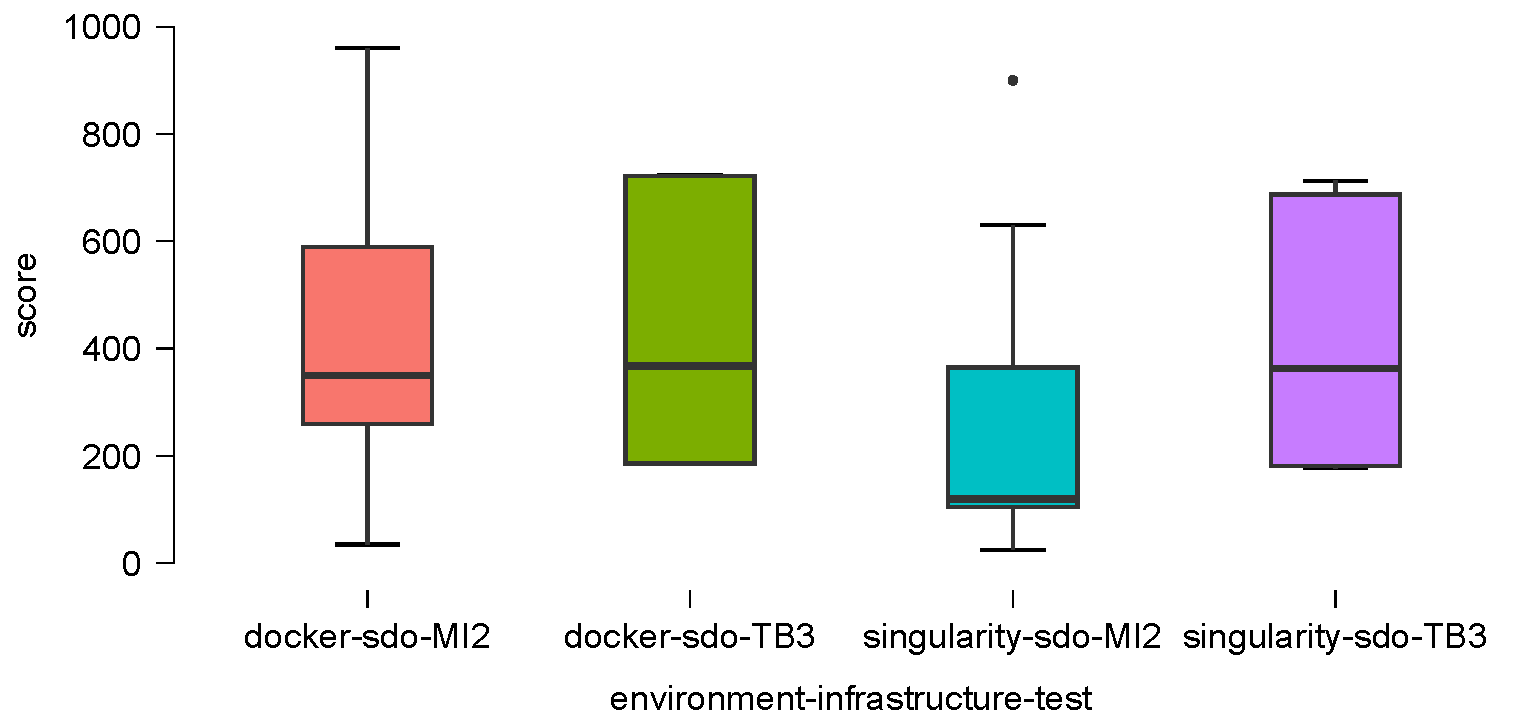
\includegraphics[width=1.05\linewidth]{./figures/data/Boxplot_VAR_score_SPLIT_enviroment-infrastructure-test_FILTER_sdo.pdf}  }
%    \caption{Comparison between sdo environments and fuzzing tests using the average score of all single-task runs.}
%    \caption{Comparativa entre entornos en sdo y pruebas de fuzzing usando el score medio de todas las ejecuciones con una unica tarea.}
%    \label{fig:Boxplot_score_sdo-evn-test}
%\end{figure*}

Secondly, the performance difference was evaluated when the singularity container is running on an HPC facility. It is commonly understood that HPC outperforms personal computers, however, it will depend on the version of the kernel, the architecture of the node, and the number of jobs. For instance, HPC systems may become outdated and lack the processing power and speed of newer computers. In addition, the architecture of the HPC system and the way it is configured can also affect its performance. As shown in Figure~\ref{fig:Barplot_score_by_paralell-unique_hpc}, we can observe that an SDO computer outperforms a single HPC node. 


%%Source: Pruebas_environment-infrastructure-test-subtype_score_hpc_uniq-paralell_sdo_uniq.csv

% 

%\begin{figure*}[ht!]
%%https://www.overleaf.com/learn/latex/Positioning_of_Figures
    \centerline{
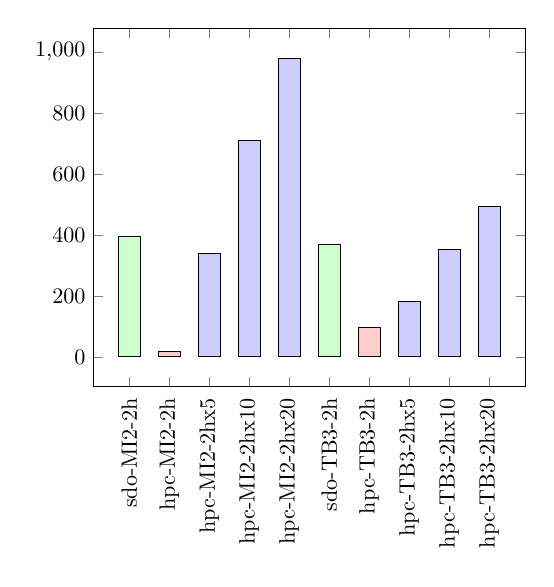
\begin{tikzpicture}[scale=0.80]
\begin{axis}[
    symbolic x coords={sdo-MI2-2h,hpc-MI2-2h, hpc-MI2-2hx5, hpc-MI2-2hx10, hpc-MI2-2hx20, sdo-TB3-2h, hpc-TB3-2h, hpc-TB3-2hx5, hpc-TB3-2hx10, hpc-TB3-2hx20},
    bar width=10pt,
    xtick=data,
    x tick label style={rotate=90, anchor=east , inner sep=5pt}]
    \addplot[ybar,fill=blue!20] coordinates {
        (sdo-MI2-2h,0)  %% Workaround: para tener leyenda en el eje x
        (hpc-MI2-2h,0)  %% Workaround: para tener leyenda en el eje x
        (hpc-MI2-2hx5,340)
        (hpc-MI2-2hx10,710)
        (hpc-MI2-2hx20,980)
        (sdo-TB3-2h,0)  %% Workaround: para tener ejex en el eje x
        (hpc-TB3-2h,0)  %% Workaround: para tener ejex en el eje x
        (hpc-TB3-2hx5,183)
        (hpc-TB3-2hx10,353)
        (hpc-TB3-2hx20,494)
    };
     %\addlegendentry{Paralell task}
    \addplot[ybar,fill=red!20] coordinates {
        (sdo-MI2-2h,0)  %% Workaround: para tener leyenda en el eje x
        (hpc-MI2-2h,16.666666671)
        (sdo-TB3-2h,0)  %% Workaround: para tener ejex en el eje x
        (hpc-TB3-2h,96.333333331)
    };
    \addplot[ybar,fill=green!20] coordinates {
        (sdo-MI2-2h,395)
        (sdo-TB3-2h,367.6666667)
    };
    
    %\addlegendentry{Unique task}
    
\end{axis}
\end{tikzpicture}}
    % El contenido de legendbox se cambia en package.tex linea 55 donde se define el robustcommand usado para dibujarlo.
%    \caption{The diagram presents a comparison between: \legendbox{green} the average score of 2h single tasks using a standalone computer (sdo), \legendbox{red} the average score of 2h single tasks using the singularity environment in the HPC infrastructure, and \legendbox{blue} parallel tasks using the score accumulated by the n parallel jobs in the HPC.}
%    %\caption{Comparativa entre tareas paralelas  \legendbox{blue} usando el score acumulado por las n tareas paraleleas  y el socre medio de tareas unicas de 2h \legendbox{red}  usando el entorno singularity en la infraestructura de HPC. Y el score medio de 2h en tareas unicas \legendbox{green} usando sdo.}
%    \label{fig:Barplot_score_by_paralell-unique_hpc}
%\end{figure*}
Finally, to determine the optimal number of jobs needed to achieve the same level of performance as a new-generation computer, additional experiments were necessary. Although previous data has shown that HPC systems can outperform new-generation computers under certain workloads, the specific conditions under which this is true are not reproduced here. Therefore, the same experiment was conducted with 5, 10, and 20 jobs. 
The MI2 results achieve almost the same performance with 5 jobs and far exceed it with 10 or 20 jobs. However, the same is not true for the TB3 tests, where 10 jobs are required to achieve similar performance and 20 jobs show no more than a 25\% increase in score. 

\section{Discussion}
\label{sec:lessons}

This section details several problems encountered in the course of the development of this work. These issues are related to the size of the container image, delays in the container executions, concurrency problems anomalies detected.

\textbf{Image size was too large} \newline
The first issue found was the Robofuzz image size was too large. So, the first step was to take advantage of the properties of Singularity, and a fixed based on a read-only file system is proposed, with a directory mapping between the container and the host that uses a unique identifier for each execution. This approach reduces the size of the image from 22.7GB in the Docker image to 7.3GB in the Singularity image and allows the entire execution context of RoboFuzz and ROS2 to be stored independently and already outside the container. This approach allows the clean-up of previous execution traces and the reuse the same container. 


\textbf{Delay between the stop order and its execution} \newline
The Slurm queue manager used in the HPC has a delay of between 10 seconds and one minute to finish container executions: To improve the accuracy of the benchmark fuzzing, the timeout command was used to define a time limit for the execution of the main command passed as a parameter. It is also used to precisely control the times in the tests using docker.
The time it takes for a job to stop from the moment it is triggered, as defined at job creation until all its processes are completed or killed on the nodes, can range from 10 seconds to more than a minute. To address this issue, a command was added as part of the execution of each fuzzing process to be measured (timeout), which runs in the same context as the fuzzer. Once the specified time has elapsed, the command terminates or analyzes the process (since it is the process's child, it is the one that invokes it with milliseconds). 

This problem also occurred with Docker and Singularity, where it could take a long time from the time the container was given the stop command until it stopped.

\textbf{The graphic session dependency} \newline
A regular graphical session is required to run some RoboFuzz examples. This limitation of the docker container, or its use in native, has been solved by using the QT library and VNC as a backend. This approach allows tests and scripts that require a graphical session to be used in a scalable way in environments without traditional graphical sessions. Standard screen output using slurm + singularity in the HPC infrastructure does not work for some crawlers that gather output using Python. A Python directive was used to disable the use of buffers and write the data on the fly to a file mapped to the host directory, with a unique path in each instance to avoid concurrency.

\textbf{Concurrency of files and blocking permissions.} \newline
The permissions for directory bindings in Docker do not work properly. To run a script and output results we propose a script added in a variable and passed as part of the instantiate command. 

\textbf{Identified anomalies} \newline
The following anomalies have been found during testing:
\begin{itemize}
    \item Docker test pts/fs-mark performance: Due to limitations with unprivileged containers, it is not possible to run some of the Phoronix Test Suite (pts) tests.
    \item Unstable RoboFuzz MI2 test: After two hours of execution, the MI2 test that implements the RoboFuzz example fuzzing tests for MoveIt 2 + Pandas becomes unstable. Further work will explore these issues looking for long-term tests. 
    \item Performance difference between the SDO and HPC jobs Linux kernel: The SDO Linux kernel (5.3.11-100.x86\_64) is more modern than the HPC Linux kernel (3.10.0-1062.9.1.x86\_64), with almost 5 times more compute performance and almost 3 times more memory performance. The main cause is how the latest kernel versions patch security vulnerabilities in Intel processors and performance improvements in container handling. 
       
\end{itemize}

The results show that the system configuration, the applications, and the type of robot have a great impact on the system performance. Starting with 20 HPC jobs characterized by the hardware presented here, the proposed H1 is confirmed. However, it is not possible to say the same with the lower number of jobs considering the proposed fuzzing flow. 

\section{Conclusions}
\label{sec:conclusions}

In conclusion, High-Performance Computing can significantly improve the fuzzing testing process by providing the necessary computational resources, parallel processing capabilities, and advanced algorithms to more efficiently and effectively explore the input space of complex systems, such as robotic software. 

The latest kernels offer significantly better performance than older ones thanks to improvements in container management and patching of processor vulnerabilities. However, parallelization, by splitting the workload across multiple threads, can significantly reduce the time it takes to complete a task.
  
\bibliographystyle{spmpsci}
\bibliography{bibliography}

\newpage

\end{document}